\section{Communication Architecture}

%%% Texto introductorio (otra vez) :v



%%%%%%%% SI SU FRENTE TIENE EL TIPO DE LA SECCION, LO AGREGAN :p
\subsection{Synchronous Communication}

% ------------------------- Payments and Refunds -------------------------
\subsubsection{Payments and Refunds}
\label{sec:pay-sync}

Synchronous calls are used only when the caller needs the answer to continue:
\begin{itemize}
  \item \textbf{Reservation $\rightarrow$ Payment Coordination}
    (\texttt{POST} \url{/api/v1/payments}): the guest is waiting to know if the
    money was held; timeout of about 1\,s and idempotent.
  \item \textbf{Reservation or support agent $\rightarrow$ Payment
    Coordination} (\texttt{POST} \url{/api/v1/refunds}): the caller needs to
    know the request was accepted (\texttt{202}); the refund itself is
    processed asynchronously.
  \item \textbf{Support Service $\rightarrow$ Payment Coordination}
    (read APIs): the agent needs the current status of a case.
  \item \textbf{Payment Coordination $\rightarrow$ Audit Service}: a manual
    refund must have its audit record confirmed before it happens (fail
    closed).
  \item \textbf{Payment Coordination and Ledger $\rightarrow$ External
    gateway}: authorize, capture, void, refund and payout, always with the
    same idempotency key on retries.
\end{itemize}

\subsubsection{Reservation and Calendar}
REST is used when the caller needs the result to continue: the guest gets the
hold immediately (\texttt{201} or \texttt{409}), and the host gets the effective
rate when saving a listing. The service calls the Pricing Service on listing
create or edit (timeout $\approx$ 500 ms, one retry within 1.5 s) and Payment
Coordination for the payment intent (timeout $\approx$ 1 s, idempotent). Pricing
is never called on the booking path. Calls have timeouts, bounded retries with
backoff and correlation IDs.

% ------------------------- Pricing Engine -------------------------
\begingroup
\setlength{\emergencystretch}{3em}
\subsubsection{Pricing Engine}
\label{sec:price-sync}

\begin{itemize}
  \item \textbf{Reservation $\rightarrow$ Pricing Service}
    (\texttt{POST} \url{/api/v1/pricing/multiplier}): the host is waiting
    for the effective rate when saving the listing; timeout of about
    500\,ms on the caller side, target p95 of 150\,ms.
  \item \textbf{Demand Indicators $\rightarrow$ Reservation}
    (\texttt{GET} \url{/internal/v1/calendar/occupancy}): the daily job needs
    the booked and blocked nights to compute occupancy; batch, outside any
    user request, with retries.
  \item \textbf{Context Indicators $\rightarrow$ SerpAPI} (HTTPS, monthly):
    the job needs the response to store it; a failure only delays context
    data.
  \item \textbf{Admin $\rightarrow$ Pricing Service $\rightarrow$ Audit
    Service}: a model version is activated only after its audit record is
    confirmed (fail closed).
\end{itemize}
\endgroup

% ------------------------- Identity, Communication and Internal Operations -------------------------
\begingroup
\setlength{\emergencystretch}{3em}
\subsubsection{Identity, Communication and Internal Operations}
\label{sec:id-sync}

\begin{itemize}
  \item \textbf{Client $\rightarrow$ Identity \& Access} (login, refresh):
    p95 of 300\,ms for login (password hashing dominates) and 100\,ms for
    refresh. Tokens are validated locally with cached public keys (under
    5\,ms), so there is no identity call per request.
  \item \textbf{Identity \& Access $\rightarrow$ User Profile} (role and
    status at login): p95 of 100\,ms, cached up to 60\,s; it \emph{fails
    closed} if the profile cannot be verified.
  \item \textbf{Client $\leftrightarrow$ Messaging:} REST with p95 of 200\,ms
    and a WebSocket with p95 of 150\,ms; the message is stored before the
    answer.
  \item \textbf{Administration, Identity, Support, Payment Coordination,
    Pricing $\rightarrow$ Audit:} append with p95 of 150\,ms; a sensitive
    action is \emph{not confirmed} if the append cannot be confirmed.
  \item \textbf{Administration $\rightarrow$ User Profile and Reservation and
    Accommodation; Support $\rightarrow$ Reservation and Payment read APIs:}
    on demand, p95 of 200--300\,ms.
\end{itemize}

\begin{figure}[H]
  \centering
  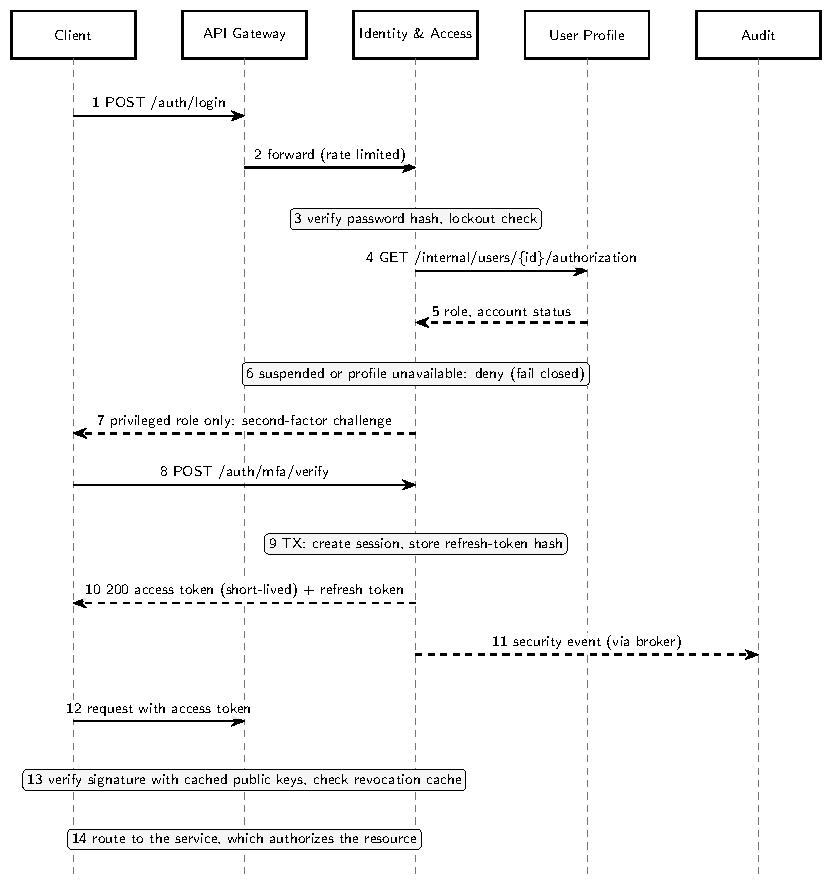
\includegraphics[width=\linewidth]{images/identity_auth_sequence.pdf}
  \caption{Log In with second factor for privileged roles, and validation of
  the access token on later requests.}
  \label{fig:id-auth}
\end{figure}

\begin{figure}[H]
  \centering
  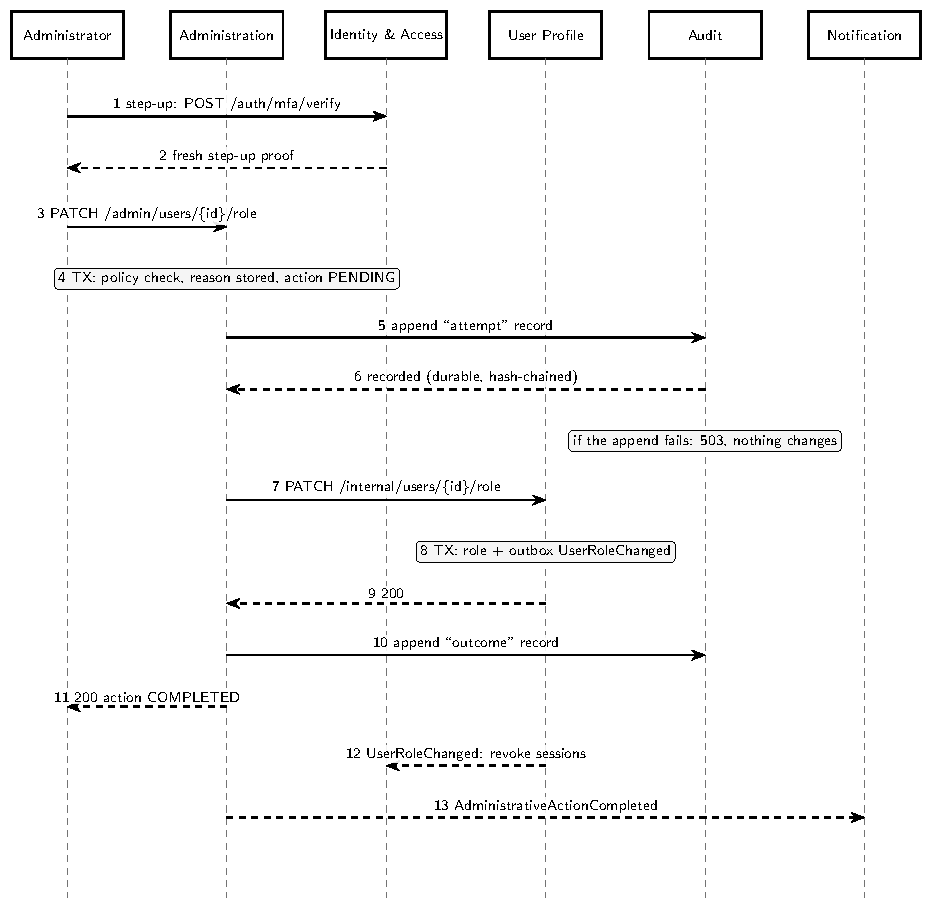
\includegraphics[width=\linewidth]{images/identity_admin_sequence.pdf}
  \caption{Manage Users: role change with step-up MFA, audit before effect,
  delegation to the owning service and session revocation.}
  \label{fig:id-admin}
\end{figure}
\endgroup

\subsection{Asynchronous Communication}
%%%% Aquí agreguen la justificación de que sea asíncrono de paso

% ------------------------- Payments and Refunds -------------------------
\begingroup
\setlength{\emergencystretch}{3em}
\subsubsection{Payments and Refunds}
\label{sec:pay-async}

Every event uses the common envelope of the platform (\texttt{eventId},
\texttt{eventType}, \texttt{eventVersion}, \texttt{occurredAt},
\texttt{producer}, \texttt{correlation\allowbreak Id}, \texttt{causationId}, payload),
is published through the outbox and delivered at least once; consumers
deduplicate on \texttt{(event\allowbreak Id, consumer\allowbreak Name)}.

\begin{longtable}{@{}L{3.6cm}L{2.4cm}L{3.2cm}L{3.8cm}@{}}
\toprule
\textbf{Event} & \textbf{Producer} & \textbf{Consumers} & \textbf{Purpose} \\
\midrule
\endhead
\texttt{Payment\allowbreak Succeeded} & Payment Coord. & Reservation, Notification &
  Money held: the reservation can be confirmed. \\
\texttt{Payment\allowbreak Failed} & Payment Coord. & Reservation, Notification &
  Declined or failed: release the dates. \\
\texttt{Payment\allowbreak Captured} & Payment Coord. & Ledger & Money charged: write
  the journal entry. \\
\texttt{Payment\allowbreak Voided} & Payment Coord. & Ledger, Audit & Hold released
  without charging. \\
\texttt{Refund\allowbreak Status\allowbreak Changed} & Payment Coord. & Ledger, Support,
  Notification, Audit & Requested, succeeded or failed refund. \\
\texttt{Payout\allowbreak Status\allowbreak Changed} & Ledger & Notification, Audit & Host payout
  scheduled, released or failed. \\
\texttt{Reservation\allowbreak Confirmed}, \texttt{Reservation\allowbreak Cancelled},
\texttt{Reservation\allowbreak Expired} & Reservation & Payment Coord., Ledger &
  Capture, void or refund, and schedule the payout. \\
\bottomrule
\caption{Events produced and consumed by Payments and Refunds.}
\label{tab:pay-events}
\end{longtable}

\paragraph{Why these interactions are asynchronous.}
\begin{itemize}
  \item \textbf{Payment results to the Reservation Service:} 3-D Secure and
    slow payment methods finish minutes after the request, so no synchronous
    caller can wait for them; the hold of 10 minutes covers that time.
  \item \textbf{Reservation events to Payment Coordination:} capture, void
    and refund depend on the reservation state, which the Reservation Service
    owns. Listening to its events avoids new synchronous calls in the booking
    path.
  \item \textbf{Events to the Ledger:} if a capture had to wait for the
    ledger, the ledger's availability would limit the booking availability
    (two services at 99.9\,\% in a chain give about 99.8\,\%).
  \item \textbf{Notifications:} an email, push or SMS failure must never make
    a payment fail.
  \item \textbf{Refund processing:} gateway refunds can take days to settle,
    so the request is accepted at once (\texttt{202}) and its result arrives as
    \texttt{Refund\allowbreak Status\allowbreak Changed}.
  \item \textbf{Gateway webhooks:} the final result of a pending payment
    arrives when the bank decides; a reconciler every 5 minutes covers lost
    webhooks.
\end{itemize}

\begin{figure}[H]
  \centering
  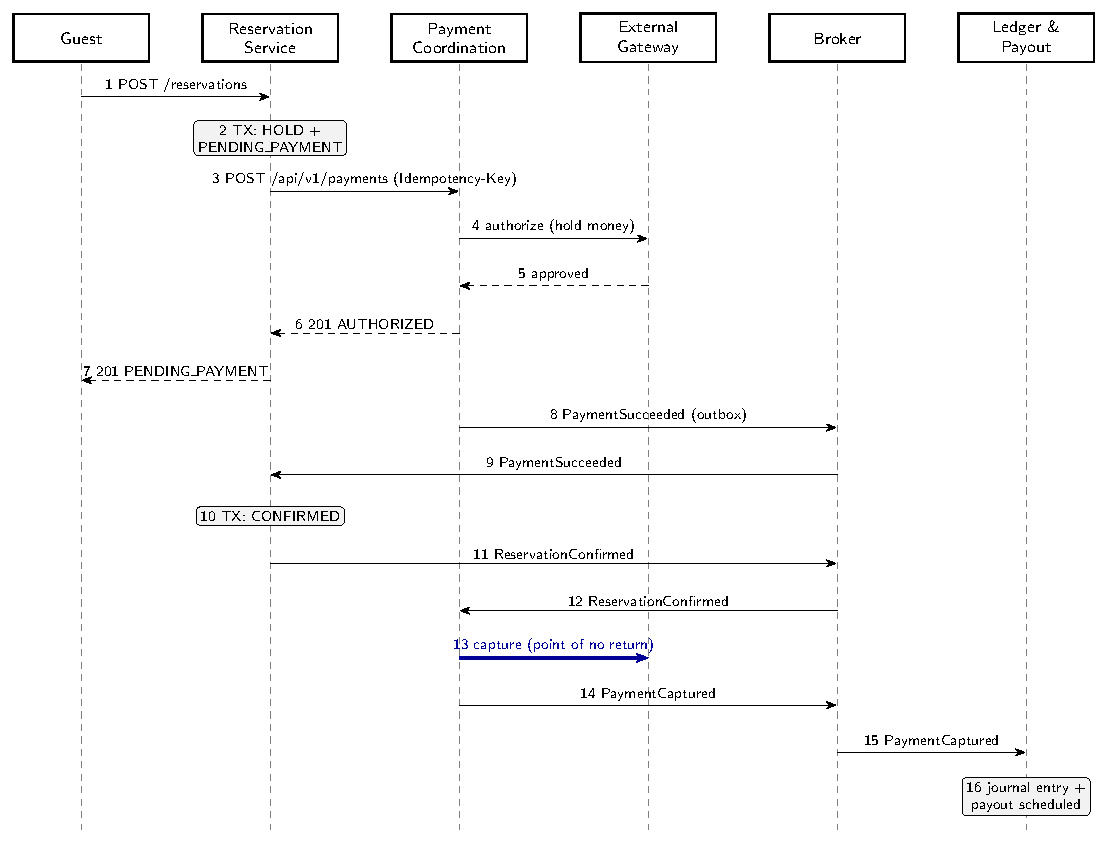
\includegraphics[width=\linewidth]{images/payments_booking_sequence.pdf}
  \caption{Booking with payment. Steps 1--10 are the booking sequence of the
  Reservation Service; steps 11--16 add the capture and the accounting.}
  \label{fig:pay-booking}
\end{figure}

\begin{figure}[H]
  \centering
  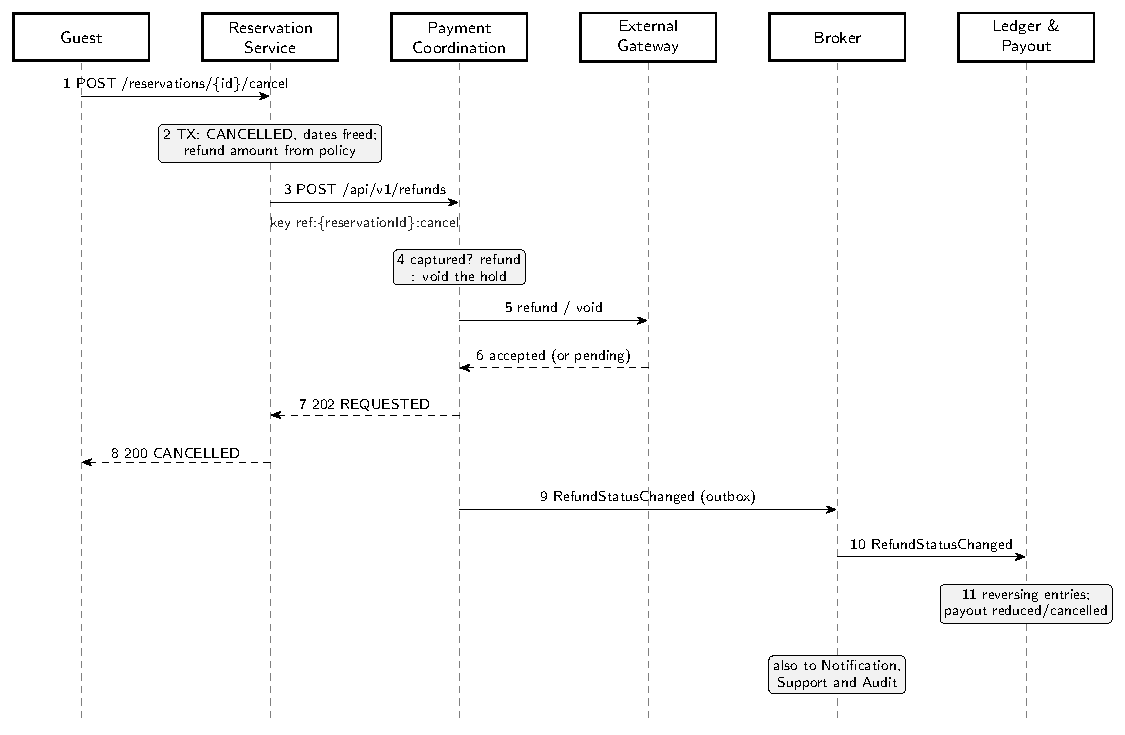
\includegraphics[width=\linewidth]{images/payments_cancel_sequence.pdf}
  \caption{Cancel Reservation with refund: void if not captured, refund
  otherwise; a failed refund does not undo the cancellation.}
  \label{fig:pay-cancel}
\end{figure}

\begin{figure}[H]
  \centering
  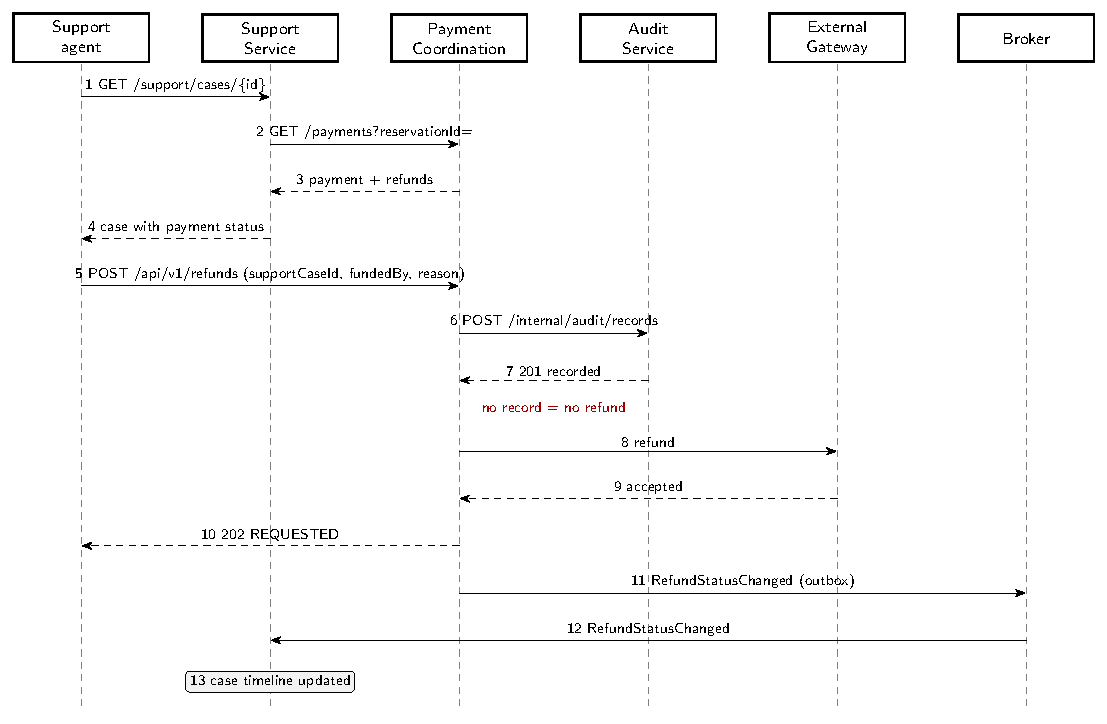
\includegraphics[width=\linewidth]{images/payments_manual_refund_sequence.pdf}
  \caption{Handle Refunds: manual refund requested by a support agent, with
  the audit record confirmed before the refund.}
  \label{fig:pay-manual}
\end{figure}

\paragraph{Failure scenarios.}
\begin{longtable}{@{}L{4.6cm}L{9.2cm}@{}}
\toprule
\textbf{Failure} & \textbf{Behaviour} \\
\midrule
\endhead
Gateway does not answer in time & The payment stays \texttt{PENDING}, never
  assumed failed; webhook or reconciler resolves it with the same key. \\
Same request retried & The idempotency record returns the original answer;
  no second charge. \\
Hold expires while the payment is pending & \texttt{Reservation\allowbreak Expired}
  makes Payment Coordination void any authorization. \\
Gateway rejects a refund & The cancellation stands;
  \texttt{Refund\allowbreak Status\allowbreak Changed} (\texttt{FAILED}) opens or updates a support
  case. \\
Audit Service unavailable & Manual refunds are not accepted (fail closed);
  automatic refunds from cancellations continue. \\
Broker down & Events wait in the outbox; payments are not blocked. \\
Duplicate webhook or event & Ignored through the inbox and the
  processed-event table. \\
\bottomrule
\caption{Failure scenarios of Payments and Refunds.}
\label{tab:pay-failures}
\end{longtable}
\endgroup

\subsubsection{Reservation and Calendar}
Events are used for work that must not delay the user: notifications, search
index refresh, audit, hold expiration and the payment result. Payment is
asynchronous because the gateway can answer after the original request; the
reservation stays \texttt{PENDING\_PAYMENT} until it arrives. Delivery is
at-least-once through a transactional outbox, with idempotent consumers and a
dead-letter queue. Published: \texttt{ReservationHeld}, \texttt{Confirmed},
\texttt{Cancelled}, \texttt{Expired}, \texttt{ReservationFlagged},
\texttt{AvailabilityChanged}, \texttt{ListingCreated}, \texttt{Updated},
\texttt{ListingDeactivated}, \texttt{AdminActionRecorded}. Consumed:
\texttt{PaymentSucceeded}, \texttt{PaymentFailed}, \texttt{HoldExpired}.

% ------------------------- Pricing Engine -------------------------
\begingroup
\setlength{\emergencystretch}{3em}
\subsubsection{Pricing Engine}
\label{sec:price-async}

\begin{longtable}{@{}L{4.0cm}L{2.6cm}L{2.6cm}L{4.3cm}@{}}
\toprule
\textbf{Event} & \textbf{Producer} & \textbf{Consumers} & \textbf{Purpose} \\
\midrule
\endhead
Search events (searches, clicks) & Search and Discovery & Demand Indicators &
  Count searches per zone and day. \\
\texttt{Demand\allowbreak Indicators\allowbreak Updated} & Demand Indicators & Pricing Service &
  Refresh occupancy, booking pace and search index of a zone. \\
\texttt{Context\allowbreak Indicators\allowbreak Updated} & Context Indicators & Pricing Service &
  Refresh the context score of a zone. \\
\bottomrule
\caption{Events produced and consumed by the Pricing Engine.}
\label{tab:price-events}
\end{longtable}

\paragraph{Why these interactions are asynchronous.}
\begin{itemize}
  \item \textbf{Search events:} searches are 60\,\% of the traffic; if each
    search had to call the engine, its latency and availability would limit
    search.
  \item \textbf{Indicator updates:} if the multiplier request called the
    indicator services (or SerpAPI) synchronously, a listing save would
    depend on three more services and an external API inside a 500\,ms
    budget. Precomputed snapshots keep the request to one local read.
\end{itemize}

\begin{figure}[H]
  \centering
  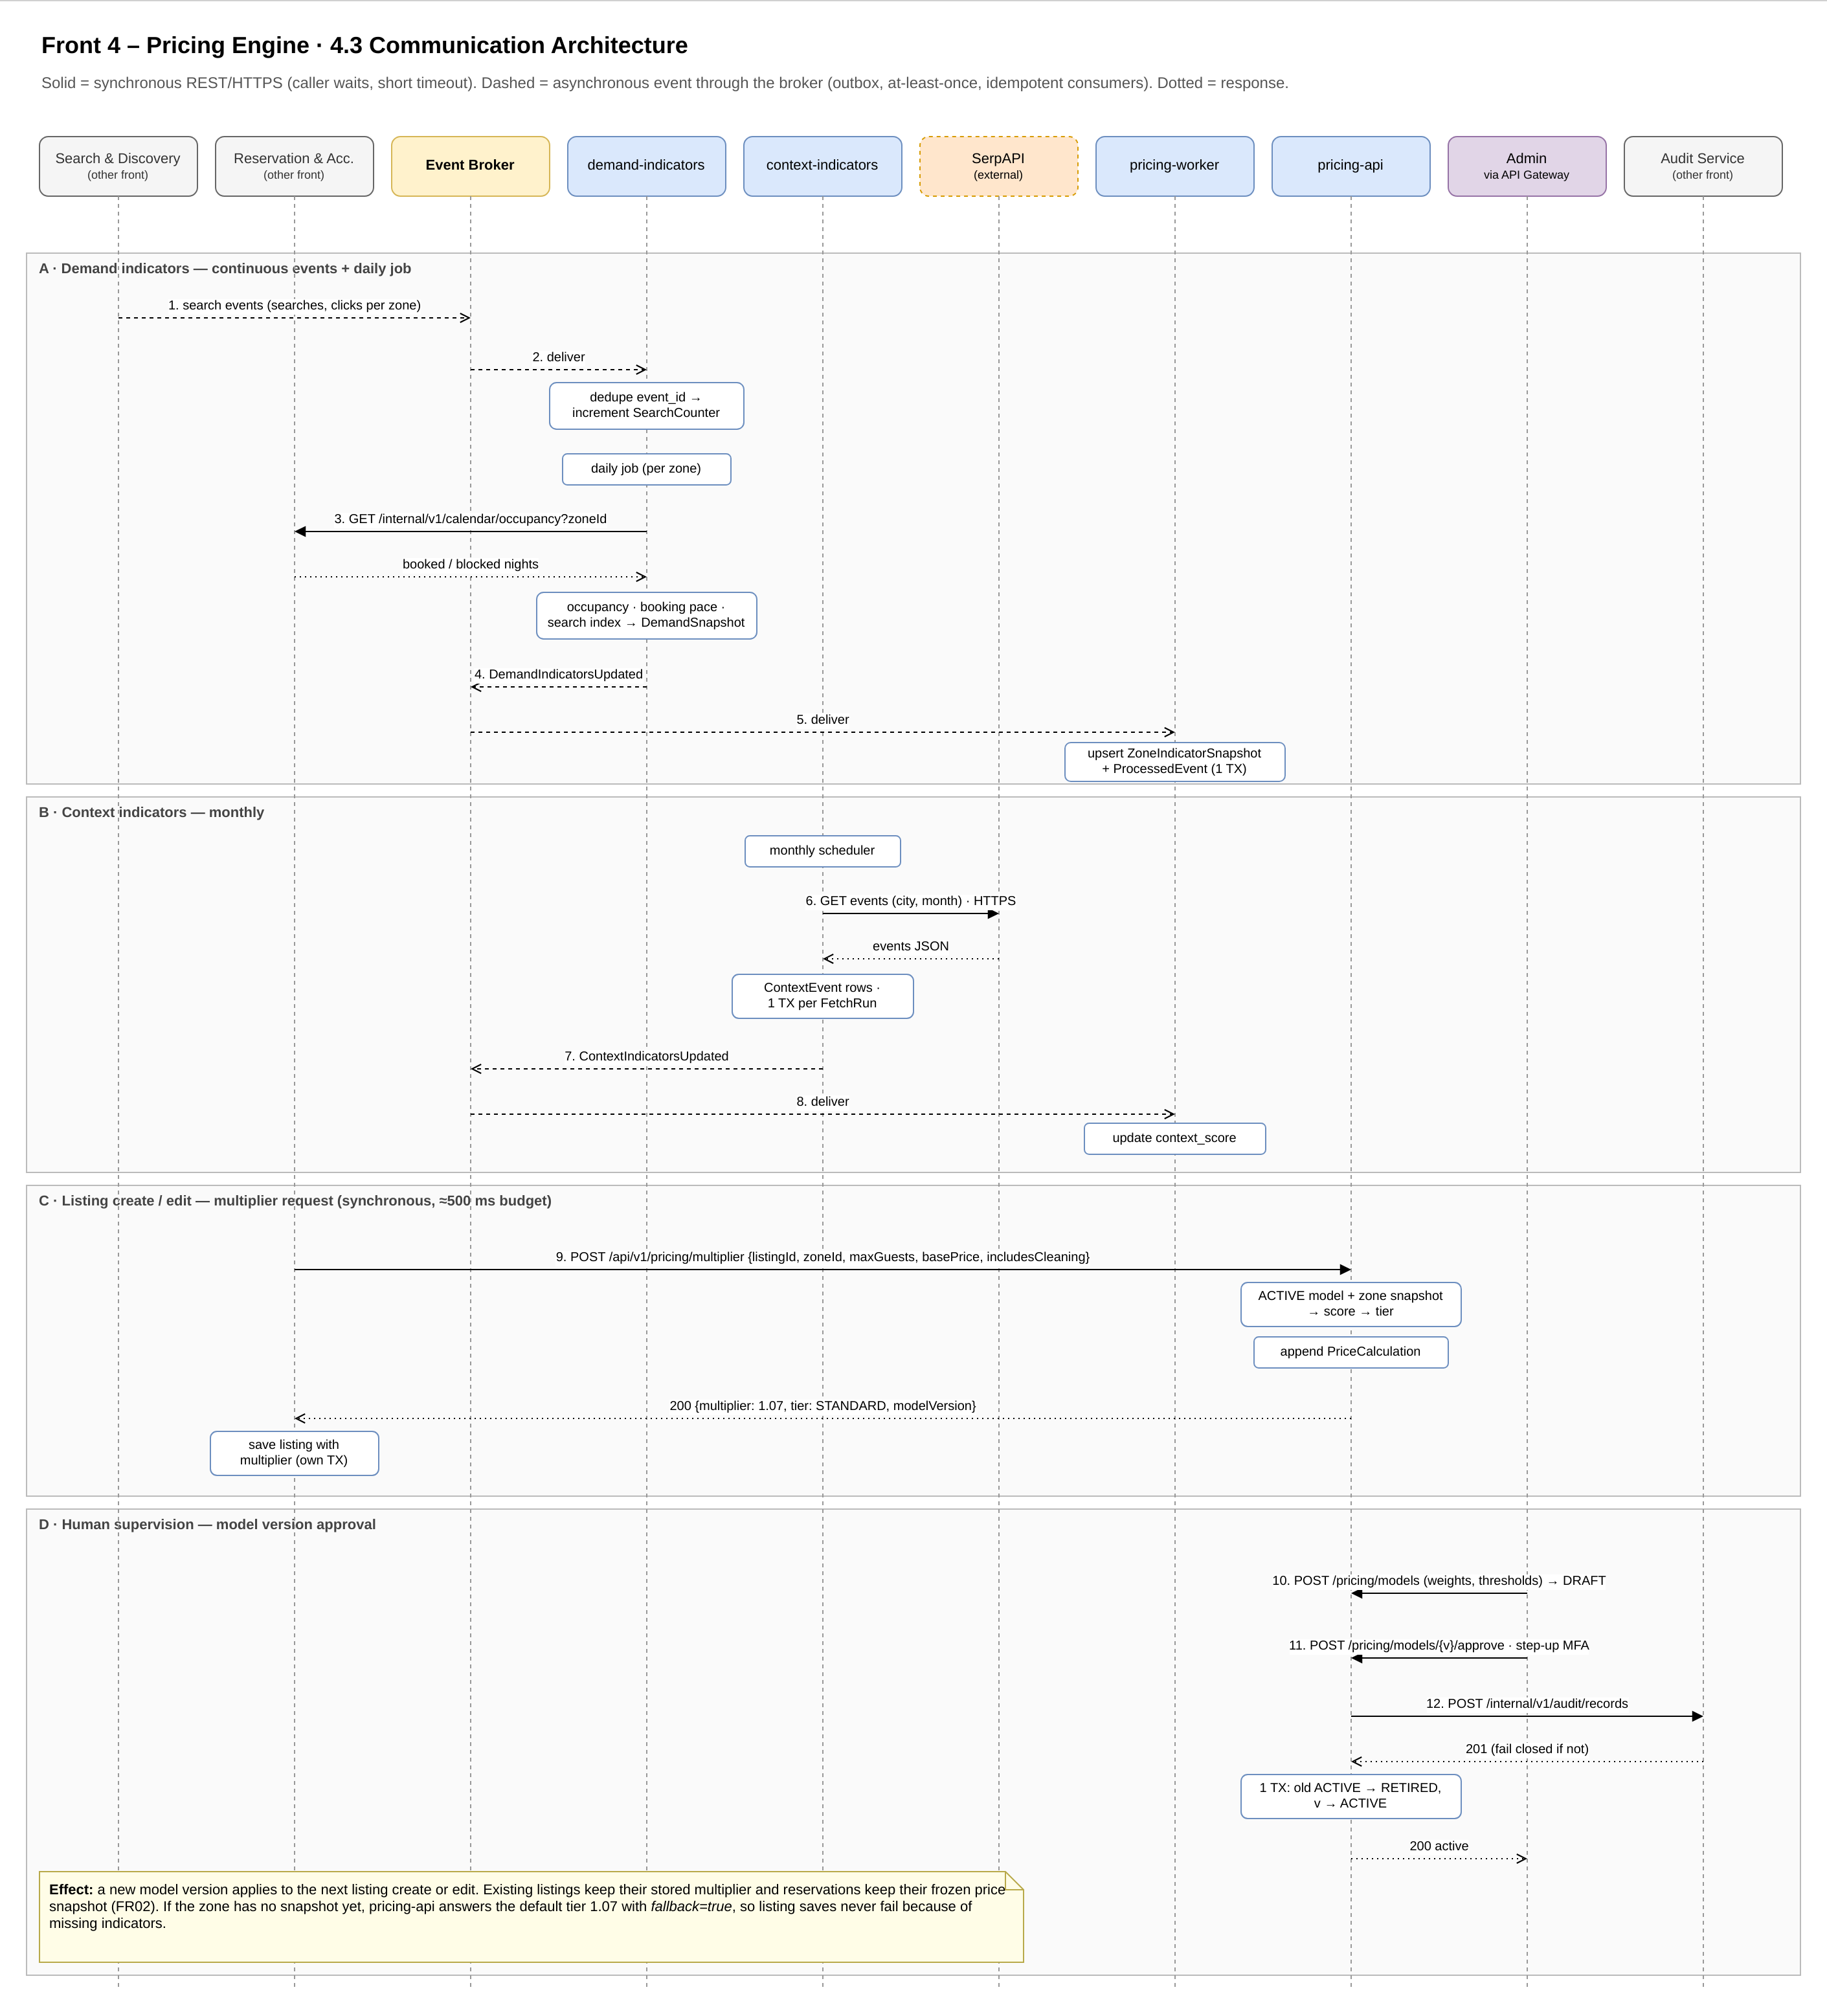
\includegraphics[width=\linewidth]{images/pricing_43_communication.png}
  \caption{Pricing Engine flows: (A) demand indicators, (B) monthly context
  refresh, (C) multiplier request on listing create or edit, (D) model
  version approval. Source: page 4.3 of \texttt{AirbnbCC.drawio}.}
  \label{fig:price-sequence}
\end{figure}

\paragraph{Failure scenarios.}
\begin{longtable}{@{}L{4.6cm}L{9.2cm}@{}}
\toprule
\textbf{Failure} & \textbf{Behaviour} \\
\midrule
\endhead
Zone without snapshot & Answers \texttt{STANDARD} (1.07) with
  \texttt{fallback = true}; the listing is saved. \\
Pricing Service down & The Reservation Service returns \texttt{502} and the
  host retries; bookings are not affected (pricing is not on the booking
  path). \\
Indicator services or broker down & The last snapshot keeps being used;
  events wait in the outbox. \\
SerpAPI unavailable & The monthly run is retried; previous context events
  remain valid. \\
Audit Service unavailable & The model version is not activated (fail
  closed); the current version keeps working. \\
Duplicate event & Ignored through the processed-event table. \\
\bottomrule
\caption{Failure scenarios of the Pricing Engine.}
\label{tab:price-failures}
\end{longtable}
\endgroup

% ------------------------- Identity, Communication and Internal Operations -------------------------
\begingroup
\setlength{\emergencystretch}{3em}
\subsubsection{Identity, Communication and Internal Operations}
\label{sec:id-async}

Events use the common envelope of the platform, are published through the
transactional outbox and are delivered at least once; consumers deduplicate on
\texttt{(event\allowbreak Id, consumer\allowbreak Name)}.

\begin{longtable}{@{}L{3.7cm}L{2.5cm}L{3.3cm}L{4.3cm}@{}}
\toprule
\textbf{Event} & \textbf{Producer} & \textbf{Consumers} & \textbf{Purpose} \\
\midrule
\endhead
\texttt{User\allowbreak Registered} & Identity \& Access & User Profile, Notification,
  Audit & Create the profile, send a welcome message. \\
\texttt{User\allowbreak Role\allowbreak Changed} & User Profile & Identity \& Access,
  Notification, Audit & Revoke sessions, notify the user, record the
  change. \\
\texttt{Message\allowbreak Created} & Messaging & Notification & New-message alert;
  identifiers only, no body. \\
\texttt{Support\allowbreak Case\allowbreak Created}, \texttt{Support\allowbreak Case\allowbreak Updated} &
  Support & Notification, Audit & Inform the reporter, record transitions. \\
\texttt{Admin\-istrative\allowbreak Action\allowbreak Completed} & Admin\-istration &
  Audit, Notification & Record the outcome, notify the affected user. \\
\bottomrule
\caption{Main events of the Identity, Communication and Internal Operations
work stream. The work stream also consumes the reservation, refund and
accommodation events of the other streams.}
\label{tab:id-events}
\end{longtable}

\paragraph{Why these interactions are asynchronous.} If email, push or SMS
were sent inside the request, a provider outage would fail a message, a case
creation or an administrative change; asynchronous delivery adds retries,
fallback and a dead-letter queue without touching the source operation.
Propagating a role change synchronously would turn it into a distributed
transaction and slow down login, so events plus short token lifetimes and
revocation are used. Audit indexing is asynchronous because the index is
derived and rebuildable.

\paragraph{Notification delivery.}
\begin{itemize}
  \item \textbf{No duplicates:} each notification has the key
    \texttt{(eventId, userId, channel)}, inserted in the same local
    transaction as the outbound task; a repeated delivery finds the key and is
    discarded.
  \item \textbf{Failures:} transient errors are retried with exponential
    backoff and jitter; permanent ones (invalid address, expired device,
    withdrawn consent) are not.
  \item \textbf{Fallback:} if push fails, email is tried when the user
    consented; one failing channel never blocks another.
  \item \textbf{Exhausted retries:} the task goes to a dead-letter queue where
    it can be inspected and replayed.
\end{itemize}

\begin{figure}[H]
  \centering
  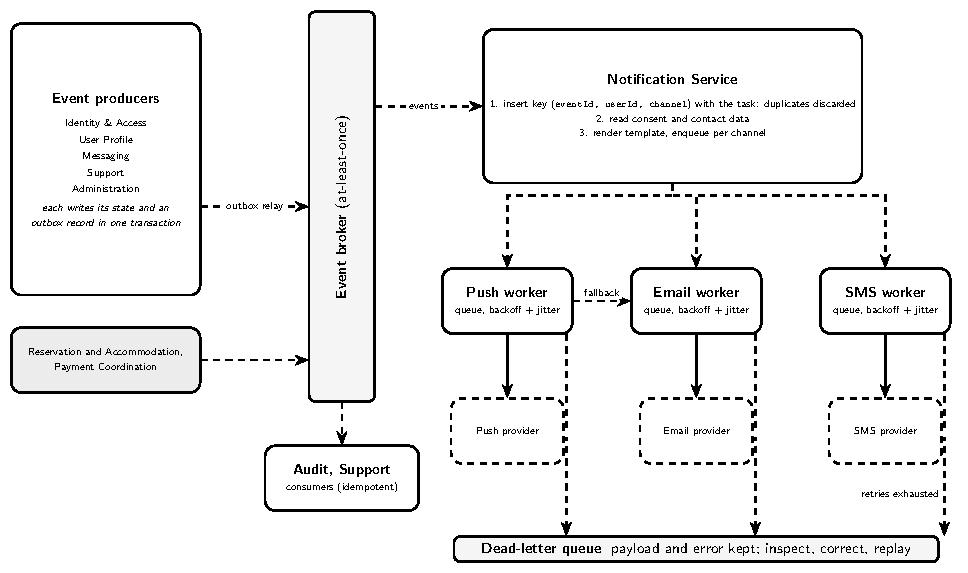
\includegraphics[width=\linewidth]{images/identity_event_flow.pdf}
  \caption{Event flow and notification pipeline: outbox relay, broker,
  duplicate suppression, per-channel workers with retries, fallback and
  dead-letter queue. The dashed boxes are external providers.}
  \label{fig:id-events}
\end{figure}

\begin{figure}[H]
  \centering
  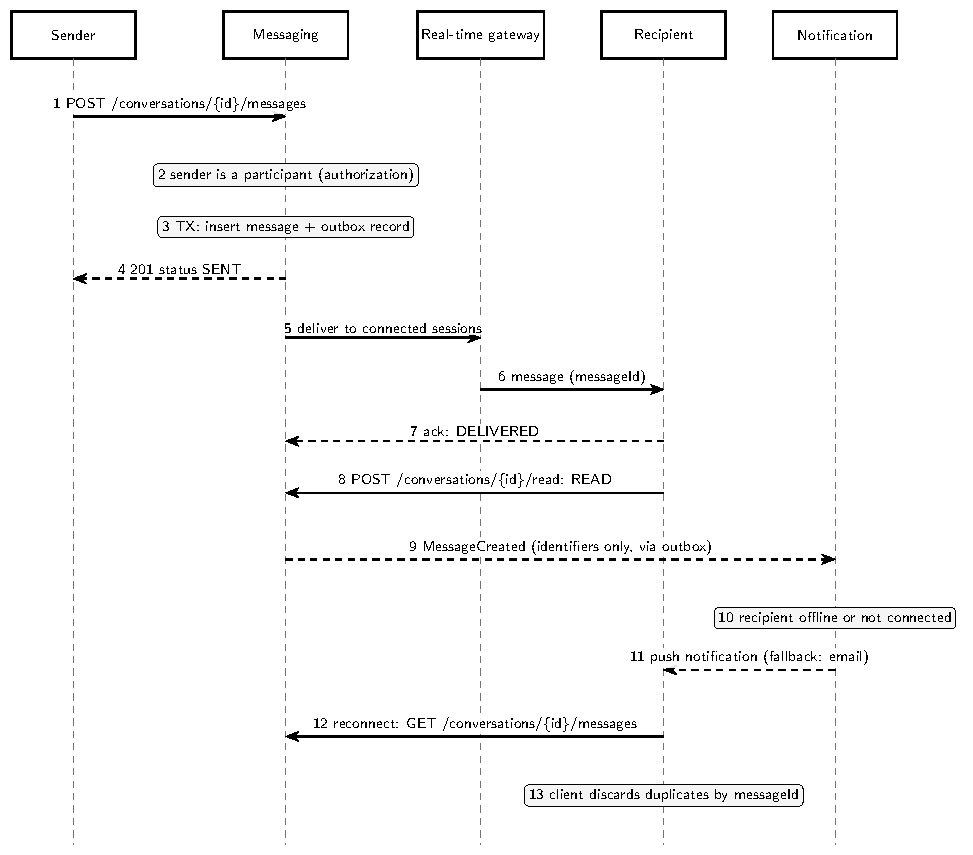
\includegraphics[width=\linewidth]{images/identity_message_sequence.pdf}
  \caption{Communicate with Host or Guest: the message is stored first, then
  delivered in real time; an offline recipient gets a push notification and
  reads the history on reconnecting.}
  \label{fig:id-message}
\end{figure}

\paragraph{Failure scenarios.}
\begin{longtable}{@{}L{4.6cm}L{9.2cm}@{}}
\toprule
\textbf{Failure} & \textbf{Behaviour} \\
\midrule
\endhead
Provider fails & The source operation is not rolled back; retries, fallback
  to another consented channel, then the dead-letter queue. \\
Duplicate event or retry & Ignored through the processed-event key and
  \texttt{(eventId, userId, channel)}. \\
Recipient offline & The message is stored; the recipient gets a push and reads
  the history on reconnecting, discarding repeats by \texttt{messageId}. \\
Audit Service unavailable & Sensitive administrative actions are not
  confirmed (fail closed); non-critical events are appended later. \\
Broker down & Events wait in the outbox; synchronous operations continue. \\
\bottomrule
\caption{Failure scenarios of the Identity, Communication and Internal
Operations work stream.}
\label{tab:id-failures}
\end{longtable}
\endgroup

\subsection{Communication Matrix}
%%%% Creo que una tablita indicando que servicios consumen que otros, está bien

% ------------------------- Payments and Refunds -------------------------
\begingroup
\setlength{\emergencystretch}{3em}
\subsubsection{Payments and Refunds}
\label{sec:pay-matrix}

\begin{longtable}{@{}L{2.3cm}L{2.3cm}L{4.0cm}L{1.6cm}L{2.5cm}@{}}
\toprule
\textbf{From} & \textbf{To} & \textbf{Operation or event} & \textbf{Pattern} & \textbf{Latency / guarantee} \\
\midrule
\endhead
Reservation & Payment Coord. & \texttt{POST /payments} (hold the money) & Sync REST & p95 $\leq$ 1\,s; idempotent \\
Reservation & Payment Coord. & \texttt{POST /refunds} after a cancellation & Sync REST (accept) & p95 300\,ms; processed async \\
Support agent (via API Gateway) & Payment Coord. & \texttt{POST /refunds} (manual) & Sync REST (accept) & p95 300\,ms; processed async \\
Support Service & Payment Coord. & Read payment and refund status & Sync REST & p95 300\,ms \\
Payment Coord. & Audit Service & Append record of a manual refund & Sync REST & Fails closed \\
Payment Coord. & External gateway & Authorize, capture, void, refund, status & Sync HTTPS & Timeout; retry with same key \\
External gateway & Payment Coord. & Webhooks (final results) & Async HTTPS & At-least-once; signed; inbox dedup \\
Payment Coord. & Reservation & \texttt{Payment\allowbreak Succeeded}, \texttt{Payment\allowbreak Failed} & Async event & At-least-once (outbox) \\
Reservation & Payment Coord. & \texttt{Reservation\allowbreak Confirmed}, \texttt{Reservation\allowbreak Cancelled}, \texttt{Reservation\allowbreak Expired} & Async event & At-least-once \\
Payment Coord. & Ledger & \texttt{Payment\allowbreak Captured}, \texttt{Refund\allowbreak Status\allowbreak Changed} & Async event & At-least-once; one entry per event \\
Reservation & Ledger & \texttt{Reservation\allowbreak Confirmed} (check-in date) & Async event & At-least-once \\
Ledger & External gateway & Host payout & Sync HTTPS & Idempotent payout key \\
Payment Coord., Ledger & Notification, Support, Audit & \texttt{Refund\allowbreak Status\allowbreak Changed}, \texttt{Payout\allowbreak Status\allowbreak Changed}, payment events & Async event & At-least-once \\
Auditor, support agent & Ledger & Balances, entries, reconciliation & Sync REST & p95 $\leq$ 1.5\,s \\
\bottomrule
\caption{Communication matrix of Payments and Refunds.}
\label{tab:pay-matrix}
\end{longtable}
\endgroup

\subsubsection{Reservation and Calendar}
\begin{table}[!ht]
  \centering
  \small
  \begin{tabularx}{\textwidth}{@{}>{\raggedright\arraybackslash}p{2.8cm}>{\raggedright\arraybackslash}p{2.8cm}>{\raggedright\arraybackslash}X>{\raggedright\arraybackslash}p{2.0cm}@{}}
    \toprule
    \textbf{From} & \textbf{To} & \textbf{Operation or event} & \textbf{Pattern} \\
    \midrule
    API Gateway & Reservation and Acc. & Listings, calendar blocks, admin status, reservations, agreements & Sync REST \\
    Reservation and Acc. & Pricing Service & Multiplier request on listing create or edit & Sync REST \\
    Reservation and Acc. & Payment Coord. & Payment intent, refund & Sync REST \\
    Pricing Service & Reservation and Acc. & Occupancy query & Sync REST \\
    Payment Coord. & Reservation and Acc. & \texttt{PaymentSucceeded}, \texttt{PaymentFailed} & Async event \\
    Scheduler & Reservation and Acc. & \texttt{HoldExpired} & Async message \\
    Reservation and Acc. & Notification & Reservation lifecycle events & Async event \\
    Reservation and Acc. & Search & Listing events, \texttt{AvailabilityChanged} & Async event \\
    Reservation and Acc. & Support and Admin. & \texttt{ReservationFlagged}, \texttt{AdminActionRecorded} & Async event \\
    \bottomrule
  \end{tabularx}
  \caption{Communication matrix of the Reservation and Accommodation Service.}
\end{table}

% ------------------------- Pricing Engine -------------------------
\begingroup
\setlength{\emergencystretch}{3em}
\subsubsection{Pricing Engine}
\label{sec:price-matrix}

\begin{longtable}{@{}L{2.4cm}L{2.4cm}L{4.0cm}L{1.6cm}L{2.4cm}@{}}
\toprule
\textbf{From} & \textbf{To} & \textbf{Operation or event} & \textbf{Pattern} & \textbf{Latency / guarantee} \\
\midrule
\endhead
Reservation and Acc. & Pricing Service & \texttt{POST} \url{/pricing/multiplier} & Sync REST & p95 150\,ms; idempotent \\
Demand Indicators & Reservation and Acc. & Calendar occupancy per zone (daily) & Sync REST & Batch; retries \\
Context Indicators & SerpAPI & Events by city and month & Sync HTTPS & Monthly; retries \\
Admin (via API Gateway) & Pricing Service & Create, approve model version & Sync REST & p95 300\,ms \\
Pricing Service & Audit Service & Append record of model activation & Sync REST & Fails closed \\
Host, admin (via API Gateway) & Pricing Service & Calculation history of a listing & Sync REST & p95 300\,ms \\
Search and Discovery & Demand Indicators & Search events & Async event & At-least-once \\
Demand Indicators & Pricing Service & \texttt{Demand\allowbreak Indicators\allowbreak Updated} & Async event & At-least-once (outbox) \\
Context Indicators & Pricing Service & \texttt{Context\allowbreak Indicators\allowbreak Updated} & Async event & At-least-once (outbox) \\
\bottomrule
\caption{Communication matrix of the Pricing Engine.}
\label{tab:price-matrix}
\end{longtable}
\endgroup

% ------------------------- Identity, Communication and Internal Operations -------------------------
\begingroup
\setlength{\emergencystretch}{3em}
\subsubsection{Identity, Communication and Internal Operations}
\label{sec:id-matrix}

\begin{longtable}{@{}L{2.3cm}L{2.3cm}L{4.0cm}L{1.6cm}L{2.5cm}@{}}
\toprule
\textbf{From} & \textbf{To} & \textbf{Operation or event} & \textbf{Pattern} & \textbf{Latency / guarantee} \\
\midrule
\endhead
Client (via API Gateway) & Identity \& Access & Login, refresh, logout & Sync REST & p95 300\,ms (login), 100\,ms (refresh) \\
API Gateway, services & Identity \& Access (keys) & Token validation with cached public keys & Local check & $<$ 5\,ms; revocation cache \\
Client & Messaging & Send, history, read state & Sync REST + WebSocket & p95 200\,ms; real time 150\,ms \\
Identity \& Access & User Profile & Role and status at login & Sync REST & p95 100\,ms; cached 60\,s; fails closed \\
Messaging, Notification & User Profile & Display and contact data & Sync REST & p95 150\,ms; cached \\
Messaging & Object storage & Upload and download URLs & Sync HTTPS & $<$ 1\,s \\
Admin\-istration & User Profile & Change role or status & Sync REST & p95 200\,ms \\
Admin\-istration & Reservation and Acc. & \texttt{PATCH} \url{/admin/listings/{id}/status} & Sync REST & p95 300\,ms; completion by event \\
Support & Reservation, Payment Coord. & Read case context, refund status & Sync REST & p95 300\,ms \\
Admin\-istration, Identity, Support, Payments, Pricing & Audit & Append a record & Sync REST & p95 150\,ms; fails closed \\
Auditor (via API Gateway) & Audit & Query records, proofs & Sync REST & Read-only \\
Any producer & Event broker & Domain events (outbox) & Async event & At-least-once; p95 $<$ 100\,ms to the broker \\
Event broker & Notification, Audit, Support, Profile, Identity & Event delivery & Async event & At-least-once; backoff; dead-letter queue \\
Notification & Providers & Email, push, SMS & Async queue + provider API & At-least-once; backoff; fallback; dead-letter queue \\
Audit & Search index & \texttt{Audit\allowbreak Record\allowbreak Appended} & Async event & Eventual; rebuildable \\
Audit & Append-only store & Persist a record or an anchor & Sync & Durable before acknowledging \\
\bottomrule
\caption{Communication matrix of the Identity, Communication and Internal
Operations work stream.}
\label{tab:id-matrix}
\end{longtable}
\endgroup

